\documentclass[t]{beamer}


%useful packages
\usepackage{color,soul}
\usepackage{amsmath,amsthm,amscd,amssymb,bm}
\usepackage{hyperref}
\usepackage[utf8]{inputenc}
\usepackage{enumerate}
\usepackage{xcolor}


%personal definitions and commands
\newcommand{\R}{\mathbb{R}} 
\newcommand{\E}{\mathbb{E}}
\newcommand{\V}{\mathbb{V}}
\newcommand{\C}{\mathbb{C}}
\newcommand{\Prob}{\mathbb{P}}
\newcommand{\e}{\epsilon}
\newcommand\numberthis{\addtocounter{equation}{1}\tag{\theequation}} %allows numbering of single equations in align* environment
\newcommand{\mtx}[1]{\ensuremath{\bm{\mathit{#1}}}}
\newcommand{\B}{\hat{\boldsymbol{\beta}}}
\newcommand{\Cov}{\mathbb{C}\text{ov}}
\newcommand{\N}{\mathcal{N}}


% \usepackage{beamerthemesplit} // Activate for custom appearance

\title{Chatterjee (2018), `Market Power and Spatial Competition in Rural India'}
\author{Nishaad Rao and Anirudh Yadav}
\date{\today}

\begin{document}

\frame{\titlepage}

\frame{\frametitle{Outline}
  \begin{enumerate}    
  \item Motivation and overview
  \item Reduced-form evidence
  \item Model
  \item Counterfactuals 
  \end{enumerate}
}


\frame{\frametitle{Motivation}
\begin{itemize}
\item Indian farmers are very poor (medium annual income $\approx \$365$).
\pause
\item Low farmer revenue partly due to the low prices they receive
\pause
\item Intermediaries (main buyers of crops) have monopsony power due to government regulations
\pause
\item Farmers are mandated to sell crops to licensed intermediaries at government-designated marketplaces \textit{in their own state}.
\end{itemize}
}

\frame{\frametitle{Questions}
\begin{enumerate}
\item Does more spatial competition between intermediaries raise farmer prices? \uncover<2->{\textbf{Yes.}}
\item How does removing the interstate trade restriction affect farmer prices/incomes/production? \\
\uncover<3->{\textbf{prices} $\uparrow$ \textbf{11\%}, \textbf{output} $\uparrow$ \textbf{7\%} }
\end{enumerate}
}

\frame{\frametitle{Institutional setting}
\begin{itemize}
\item State-level legislation (APMC Acts) mandate that the first sale of crops after harvest must be at government-designated marketplaces, and buyers must obtain a license.
\pause
\item Effectively prohibits farmers from selling crops in neighbouring states.
\pause
\item Reduces competition between marketplaces across state borders.
\pause
\item Treat each physical marketplace as having only one intermediary buyer.
\end{itemize}

}

\frame{\frametitle{Empirical methodology}
\begin{itemize}
\item Measure of spatial competition faced by a market $m$:
\begin{align*}
\text{comp}_m = \sum_{j \in \mathcal{M}/\{m\}} \left\{ \frac{1}{\text{distance}_{mj}}\right\}\bm{1}[\text{$m$ and $j$ are in the same state}]
\end{align*}
\pause
\item Analogous measure of interstate spatial competition:
\begin{align*}
\text{comp}'_m = \sum_{j \in \mathcal{M}/\{m\}} \left\{ \frac{1}{\text{distance}_{mj}}\right\}\bm{1}[\text{$m$ and $j$ not in the same state}]
\end{align*}
\end{itemize}

}

\frame{\frametitle{Example}
\begin{figure}
\centering
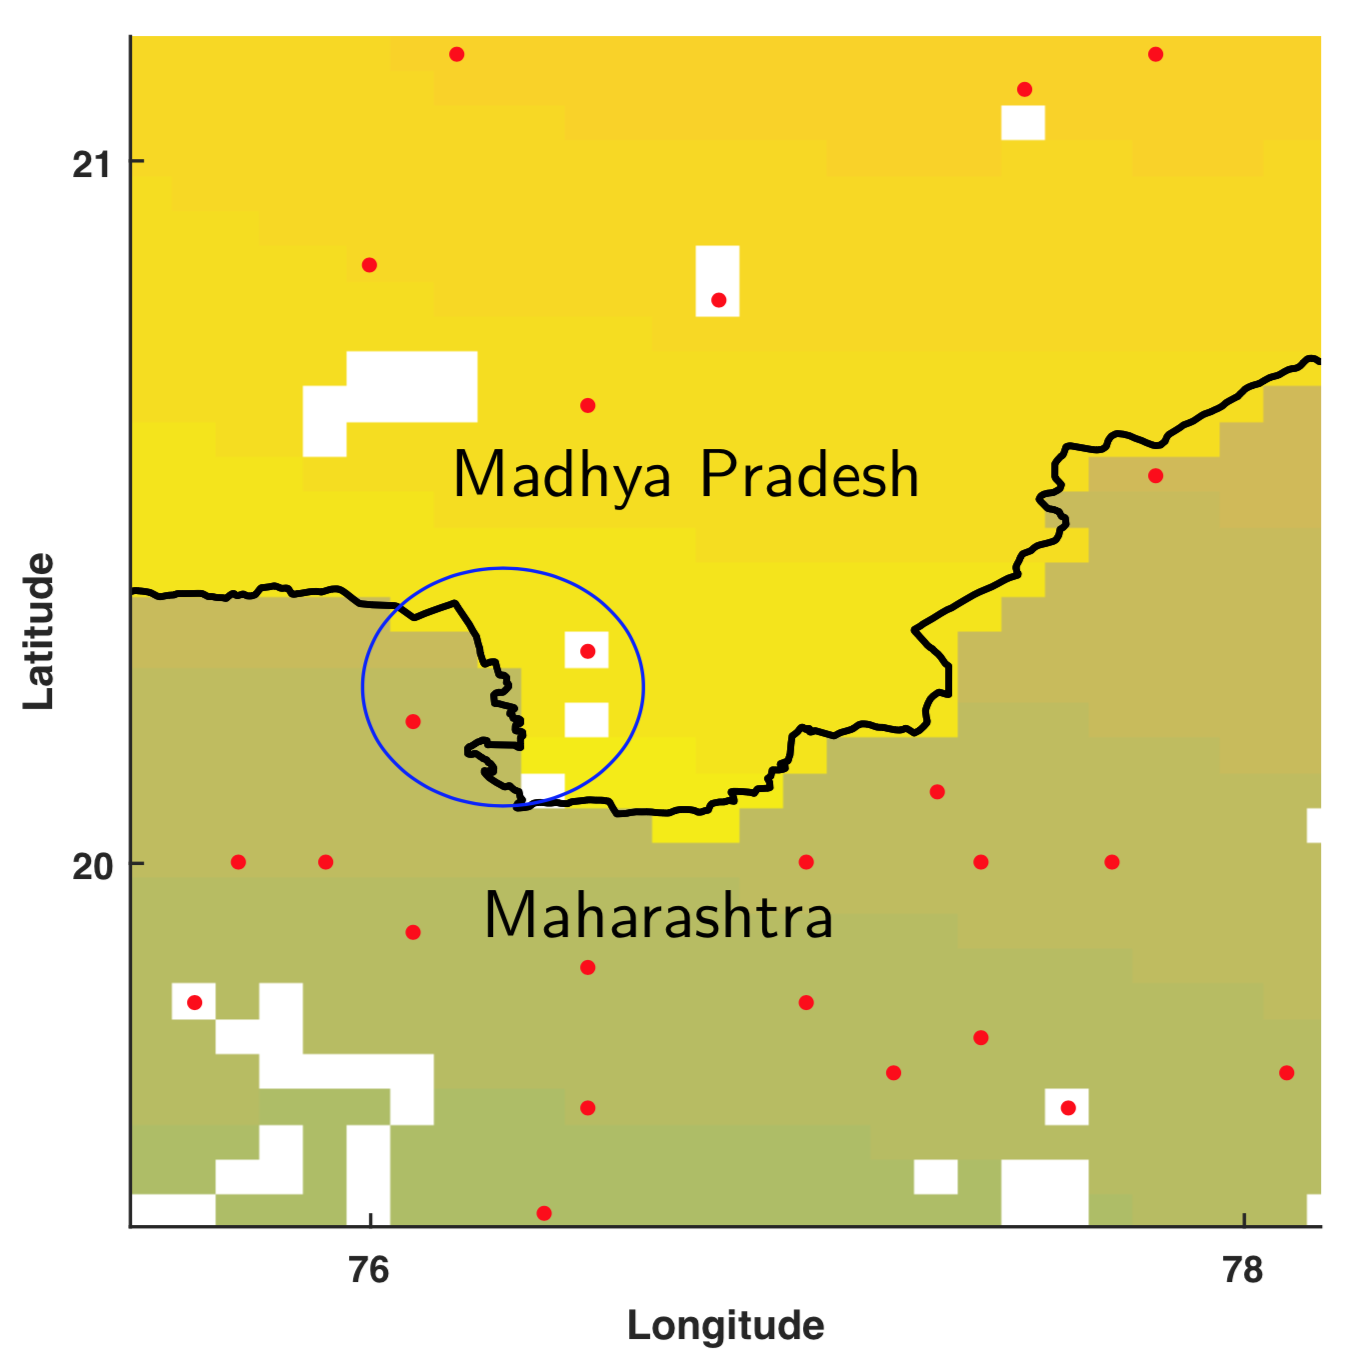
\includegraphics[width=0.7\textwidth]{example}
\end{figure}
}

\frame{\frametitle{Empirical methodology}
\begin{itemize}
\item Main specification:
\begin{align*}
\log p^f_{cmdst} =& \beta_0 + \beta_1 \text{comp}_m + \beta_2 \text{comp}'_m + \mtx{X}'_{cdt}\beta_3 \\
&+ \gamma_t + \gamma_c + \gamma_s + \e_{cmdt}
\end{align*}
where $p^f_{cmdst}$ is the price a farmer receives for crop $c$, at market $m$, in district $d$, state $s$, and month $t$.
\pause
\item Sample: 10 years (2005--2014), 2978 markets.
\end{itemize}

}

\frame{\frametitle{Empirical results}
\centering
\begin{table}
\begin{tabular}{lrr}
 & $\hat{\beta}_1$ & $\hat{\beta}_2$\\
 \hline
Point estimate &0.0163 & $-0.0005$\\
Std. err. & 0.0043 & 0.0012
\end{tabular}
\end{table}
\pause
\begin{itemize}
\item Greater spatial competition increases farmer prices!
\end{itemize}

}


\section{Appendix}
\frame{
\vfill
\centering
\usebeamerfont{title}\textbf{Appendix}
\vfill
}

\frame{\frametitle{Causal estimates}
\begin{itemize}
\item Basic idea: choose market pairs that are close together but separated by a border 
\item Factors that affect price (other than spatial competition) should be similar for the market pairs. 
\item For each market pair $(m,m')$ estimate:
\begin{align*}
\Delta \log p^f_{cmdt} = \beta_1(\Delta \text{comp}_m) + \gamma_{ss'} + \tilde \e_{cmdt}
\end{align*}
\end{itemize}

}

\frame{\frametitle{Causal estimates}
\begin{table}
\centering
\caption{Border Discontinuity Regressions}
\begin{tabular}{lrrr}
\hline
& \multicolumn{3}{c}{Distance between market pairs (km)} \\
& $<25$ & $<30$ & $<35$ \\
\hline
$\hat{\beta}_1$ &0.025 & 0.035 & 0.036\\
Robust std. err. & 0.011 & 0.013 & 0.009\\
\end{tabular}
\end{table}
}




\end{document}
